\section{Лекція 10: Функції}
 
 \subsection{Рекурсивні функції} 
\begin{frame}
% \frametitle{Логічні висновки}
Рекурсивна функція — функція, що викликає саму себе. При цьому функція розміщується в стек виклику функції. Кількість внутрішніх викликів функції називається глибиною рекурсії.
\begin{figure}
  \begin{center}
    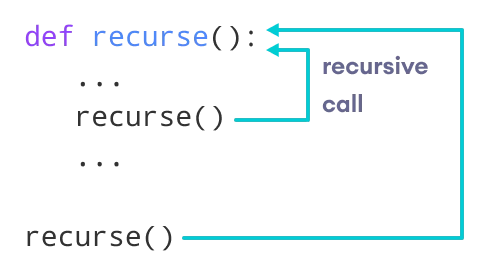
\includegraphics[width=0.5\textwidth,height=0.5\textheight]{pictures/recursion.png}
  \caption{Рекурсивна функція}
\label{function}
  \end{center}
\end{figure}
\end{frame}

\begin{frame}
% \frametitle{Логічні висновки}
Приклад рекурсивної функції:

\vspace{1cm}

\texttt{def recursive(value):}

\texttt{~~~~print(value)}

\texttt{~~~~if value < 4:}

\texttt{~~~~~~~~recursive(value)}

\texttt{~~~~print(value)}

\end{frame}

\subsection{Lambda-функції} 
\begin{frame}
% \frametitle{Логічні висновки}
Lambda-функція — анонімна функція.

\Large{\texttt{lambda param\_1, param\_2, ... : команда}}

\normalsize
\begin{itemize}
  \item lambda-функція автоматично повертає результат свого виконання (оператор return не потрібен);
  \item lambda-функція зазвичай присвоюється якійсь змінній; 
  \item lambda-функція може бути елементом будь-якої конструкції мови Python;
  \item всередині lambda-функції не можна виконувати присвоювання.
\end{itemize}

\end{frame}

\begin{frame}
% \frametitle{Логічні висновки}
Приклад використання lambda-функції:

\texttt{def get\_filter(a, filter=None):}

\texttt{~~~~ if filter is None:}

\texttt{~~~~~~~~return a}

\texttt{~~~~res = []}

\texttt{~~~~for filter in a:}

\texttt{~~~~~~~~if filter(x):}

\texttt{~~~~~~~~~~~~res.append(x)}

\texttt{~~~~return res}

\vspace*{0.8cm}

\texttt{print(get\_filter(a))}

\texttt{print(get\_filter(a, filter=lambda x: x \% 2 == 0))}
\end{frame}

\subsection{Простір імен} 
\begin{frame}
% \frametitle{Логічні висновки}
Локальний простір імен: простір імен містить локальні імена всередині функції. Цей простір імен створюється під час виклику функції і продовжується, поки функція не повернеться.

Глобальний простір імен: це простір імен, який включає імена різних імпортованих модулів, які ви використовуєте в проекті. Він створюється, коли модуль включений у проект, і існує до завершення виконання програми.

\end{frame}

\subsection{Область видимості} 
\begin{frame}
% \frametitle{Логічні висновки}
Локальна область видимості є внутрішньою областю, яка містить список локальних імен, доступних у поточній функції.

Глобальна область  видимості - область всіх функцій, що закривають. 

Пошук імені починається з найближчої області, що охоплює, і переміщається назовні.

Щоб всередині функції змінити глобальну змінну \texttt{var} використовується команда \texttt{global var}.

Щоб всередині функції працювати зі змінною \texttt{var} із зовнішнього (локального) простору імен використовується команда \texttt{nonlocal var}.

\end{frame}
